\newcommand{\rendering}[1]{
  \includegraphics[height=\renderingheight]{assets/\clogdirname/pipeline/image_#1.png}
}
\newcommand{\uvmap}[1]{
  \includegraphics[height=\uvheight]{assets/\clogdirname/pipeline/interpolation_#1.png}
}
\newcommand{\modulateduvmap}[1]{
  \includegraphics[height=\renderingheight]{assets/\clogdirname/pipeline/modulated_pred_#1.png}
}
\newcommand{\unmodulateduvmap}[1]{
  \includegraphics[height=\renderingheight]{assets/\clogdirname/pipeline/unmodulated_pred_#1.png}
}
\newcommand{\clogpipelinefig}{
  \def\inputheight{128bp}
  \def\renderingheight{64bp}
  \def\preplasheight{78bp}
  \def\uvheight{52bp}
  \centering
  \font\nullfont=cmr10
  \tikzsetnextfilename{clogpipeline}
  \tikzset{external/export next=false}
  \resizebox{\linewidth}{!}{
    \begin{tikzpicture}[
        >=stealth',
        overlay/.style={
            anchor=south west,
            draw=black,
            rectangle,
            line width=0pt,
            outer sep=0,
            inner sep=0,
          },
      ]
      \node (data) {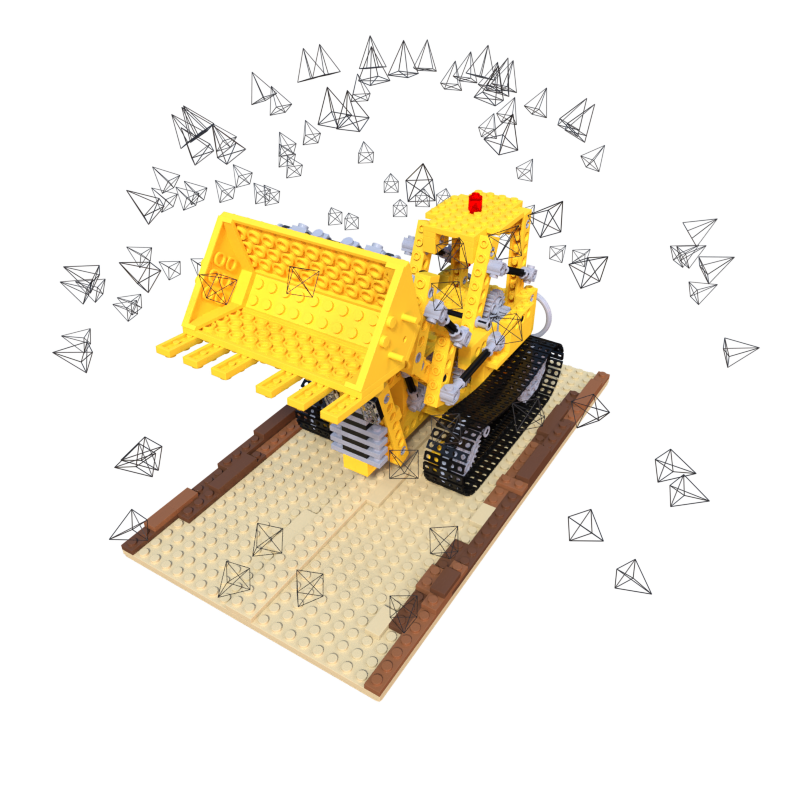
\includegraphics[height=\inputheight]{assets/\clogdirname/pipeline/vis.png}};

      \matrix[
        matrix of nodes,
        right=1em of data,
        column sep=0pt,
        row sep=1.4em,
        ampersand replacement=\&,
        inner sep=0,
        outer sep=0
      ] (pictures) {
        \rendering{0.00} \&
        \rendering{0.25} \&
        \rendering{0.50} \&
        \rendering{0.75} \&
        \rendering{1.00} \\
        \uvmap{0.00} \&
        \uvmap{0.25} \&
        \uvmap{0.50} \&
        \uvmap{0.75} \&
        \uvmap{1.00}     \\
      };
      \node[above right=0em and 0.2em of pictures-2-1.north, scale=0.4] (firstnet) {\rotatebox{90}{\usebox\neuralnet}};
      \node[above=-0.4em of firstnet.north] {\smaller \cref{eq:clog-decoders}};
      \node[above right=0em and 0.2em of pictures-2-2.north, scale=0.4]{\rotatebox{90}{\usebox\neuralnet}};
      \node[above right=0em and 0.2em of pictures-2-3.north, scale=0.4]{\rotatebox{90}{\usebox\neuralnet}};
      \node[above right=0em and 0.2em of pictures-2-4.north, scale=0.4]{\rotatebox{90}{\usebox\neuralnet}};
      \node[above right=0em and 0.2em of pictures-2-5.north, scale=0.4]{\rotatebox{90}{\usebox\neuralnet}};

      \node[right=-1em of data.west, align=center, anchor=base] (stageone) {\rotatebox{90}{Stage I}};
      \node[right=-1.5em of pictures-2-1.west, align=center]{\rotatebox{90}{\smaller Grid of Latents~$\cloglatents$}};
      \node[above=0em of data.north, align=center] {Calibrated cameras};

      \draw[-stealth,  thick, dashed,  ->] ([yshift=4pt]pictures-1-1.north west) -- node [above, midway] {\smaller Training progression and upsampling~(\cref{eq:clog-upsampling})} ([yshift=4pt]pictures-1-5.north east);

      \node[right=1em of pictures.east] (preplas) {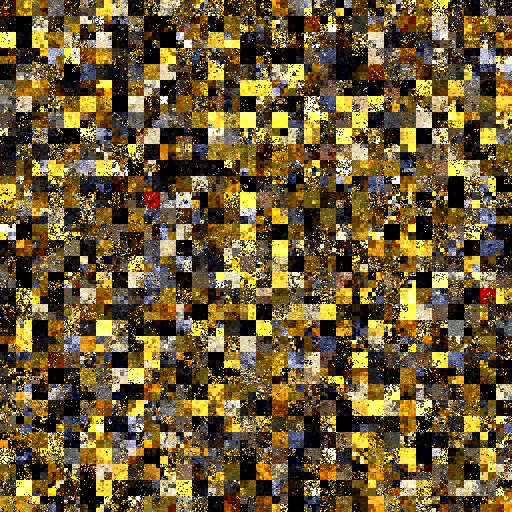
\includegraphics[height=\inputheight]{assets/\clogdirname/plas/unsorted_colors.png}};
      \node[below=3em of preplas.south] (postplas) {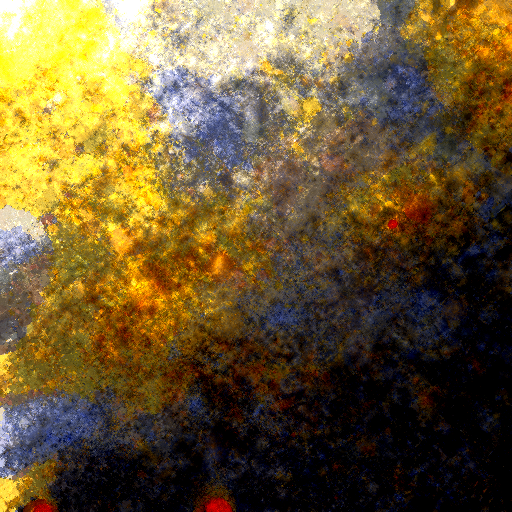
\includegraphics[height=\inputheight]{assets/\clogdirname/plas/sorted_colors.png}};k
      \node[above=0em of preplas.north, align=center] {Trained Grid};

      \draw[-stealth, shorten >= 1pt, shorten <= 1pt,  thick,  ->] (preplas.south) -- node [right, midway] {\smaller PLAS~\cite{morgenstern2024compact}}(postplas.north);

      \node[above left=0.25em and 3.5em of postplas, anchor=north east, scale=1.15] (modulator) {\rotatebox{180}{\usebox\neuralnet}};

      \matrix[
        matrix of nodes,
        left=12em of postplas.west,
        column sep=0pt,
        row sep=0em,
        ampersand replacement=\&,
        inner sep=0,
        outer sep=0
      ] (secondstage) {
        \modulateduvmap{0.00} \&
        \modulateduvmap{0.25} \&
        \modulateduvmap{0.50} \&
        \modulateduvmap{0.75} \&
        \modulateduvmap{1.00}   \\
        \unmodulateduvmap{0.00} \&
        \unmodulateduvmap{0.25} \&
        \unmodulateduvmap{0.50} \&
        \unmodulateduvmap{0.75} \&
        \unmodulateduvmap{1.00} \\
      };
      \draw[-stealth, decoration={snake, pre length=0.01mm, segment length=2mm, amplitude=0.3mm, post length=1.5mm}, decorate, thick] ([yshift=-32bp]postplas.west) -- node [above, midway] {No modulation} (secondstage-2-5);

      \draw[-stealth, decoration={snake, pre length=0.01mm, segment length=2mm, amplitude=0.3mm, post length=1.5mm}, decorate, thick] ([yshift=32bp]postplas.west) -- node [above, midway] {\cref{eq:clog-modulator}} (modulator.east);
      \draw[-stealth, decoration={snake, pre length=0.01mm, segment length=2mm, amplitude=0.3mm, post length=1.5mm}, decorate, thick] (modulator.west) -- node [above, midway] {\cref{eq:clog-modulating}} (secondstage-1-5);

      \node[above=-0.5em of modulator] {Our modulator $\modulator$};

      \node[below=18em of stageone.south, align=center, anchor=base] {\rotatebox{90}{Stage II}};

      \draw[-stealth,  thick, dashed,  ->] ([yshift=0pt]secondstage-1-5.north east) -- node [above, midway] {\smaller Decreasing LoD~$\lod\in[0, 1]$} ([yshift=0pt]secondstage-1-1.north west);

      \node[right=-1.5em of secondstage-1-1.west, align=center] {\small\rotatebox{90}{\textbf{Ours}}};
      \node[right=-1.5em of secondstage-2-1.west, align=center] {\small\rotatebox{90}{For comparison}};

    \end{tikzpicture}
  }
}
\begin{figure}
  \centering
  \clogpipelinefig
  \caption{
    \textbf{Pipeline --}
    We represent the scene with a 2D UV map containing features that an MLP
    interprets 3D Gaussians.
    We first train the UV map at the highest resolution and sort it to ensure
    spatial coherence of similar features, enabling effective subsampling.
    For any desired level of detail (LoD), we obtain the corresponding UV map
    by downsampling and processing it through a modulator that adapts the
    features to map correctly to 3D Gaussians at reduced density.
    This approach enables support for \emph{arbitrary} levels of detail.
  }
  \label{fig:clog-pipeline}
\end{figure}
\section{Method}
  \label{sec:blendifleds-method}
  % \TODO{smoother intro, describing the input data, the desired output, and
  % the meta-data the expert systems provide... tet-mesh, expression
  % parameters, etc...}

  % \ky{%
  We introduce a volumetric model that can be driven by input expressions and
  visualize it in in~\cref{fig:blendfields-pipeline}.
  We start this section by explaining our model and how we train and drive it
  with novel expressions utilizing parametric face models
  (\cref{sec:blendfields-model}).
  We then discuss how to compute measures of volume expansion and compression
  in the tetrahedra to combine volumetric models of different expressions
  (\cref{sec:blendfields-similarity}) and how we remove artifacts in
  out-of-distribution settings (\cref{sec:blendfields-smoothness}).
  We conclude this section with implementation details
  (\cref{sec:blendfields-implementation}).

  % \ve{I rewrote the previous paragraph as it did not match the rest of the
  % section after all the rewrites} }%

  \subsection{Our model}
    \label{sec:blendfields-model}
    % --- VolTeMorph
    Given a neutral expression $\template\expression$, and a collection of
    posed images $\{\pixelcolor_c\}$ of this expression from multiple views,
    \VolTeMorph employs a map~$\map$ to fetch the density and
    radiance\footnote{We omit view-dependent effects to simplify notation but
    include them in our implementation.
    } for a new expression $\expression$ from the \textit{canonical} frame defined by expression $\template\expression$:
    \begin{align}
      \radiance(\pos; \expression) & = \template\radiance(\bar\pos), \quad \bar\pos = \map(\pos; \expression \rightarrow \template\expression)
      \\
      \density(\pos; \expression)  & = \template\density(\bar\pos), \quad \bar\pos = \map(\pos; \expression \rightarrow \template\expression)
      \label{eq:blendfields-densityVoltemorph}
      \\
      \loss{rgb}                   & =
      \expect_{\pixelcolor \sim \{\pixelcolor_c\}} \:
      \expect_{\ray \sim \pixelcolor} \:
      \loss{rgb}^\ray
      \\
      \loss{rgb}^\ray              & = \| \pixelcolor(\ray; \expression) - \pixelcolor(\ray) \|_2^2,
    \end{align}
    where $\pixelcolor(\ray; \expression)$ is a pixel color produced by our model conditioned on the input expression $\expression$, $\pixelcolor(\ray)$ is the ground-truth pixel color, and the mapping~$\map$ is computed from smooth deformations of a tetrahedral mesh to render unseen expressions~$\expression$.
    % \mkc{C(r) is previously defined as color of rendered pixel, C(r,e) on the
    % other hand is not defined. Also eq. 5 is unclear to me. } \AT{(5) first
    % expectation is take a random image from the set of train images; second
    % is take a random pixel from such image (ray-pixel is 1:1)} \kk{
    We use expression vectors $\expression$ from parametric face models, such
    as FLAME~\cite{li2017flame,wood2021fake}.
    % } \AT{move up to 3.0, see note} \AT{quickly mention where $\expression$
    % comes from.}
    However, as neither density nor radiance change with $\expression$,
    changes in appearance are limited to the low-frequency deformations that
    $\map$ can express.
    For example, this model cannot capture high-frequency dynamic features
    like expression wrinkles.
    We overcome this limitation by conditioning radiance on expression.
    For this purpose, we assume radiance to be the sum of a template radiance (\ie rest pose appearance of a subject) and $\nExpr$ residual radiances (\ie details belonging to corresponding facial expressions):
    \begin{equation}
      \outputcolor(\pos; \expression) = \bar\radiance(\pos) + \sum_{k=\iExpr}^\nExpr
      \blendingweight_\iExpr(\pos; \expression)
      \cdot
      \aux\radiance_\iExpr(\pos),
      \label{eq:blendfields-multiheadradiance}
    \end{equation}
    % --- \JV{here we could draw a parallel with how blendshapes activate e.g.
    % wrinkle maps in traditional graphics pipelines}
    We call our model \textit{blend fields}, as it resembles the way in which
    blending is employed in 3D morphable models~\cite{blanz1999morphable} or
    in wrinkle maps~\cite{oat2007animated}.
    Note that we assume that pose-dependent geometry can be effectively
    modeled as {a convex combination of colors
    $[\aux\radiance(\pos)]_{\iExpr=1}^{\nExpr}$}, since we employ the same
    density fields as in~\cref{eq:blendfields-densityVoltemorph}.
    % \mkc{This comes off a little confusing as up to this point we do not
    % mention view dependent effects}
    In what follows, for convenience, we denote the vector field of blending
    coefficients as $\blendfield(\pos) {=}
    [\blendingweight_\iExpr(\pos)]_{\iExpr=1}^{\nExpr}$.
    % \ve{braces $\{\cdot \}$ are used for sets, once a set of weights are used
    % as a vector it is confusing to keep the set notation as it has no
    % ordering and algebra would not work. The text mixed the notation for sets
    % and vectors. I changed it where necessary for instance $\blendfield(\pos)
    % {=} \{\blendingweight_\iExpr(\pos)\}$ into $\blendfield(\pos) {=}
    % [\blendingweight_\iExpr(\pos)]_{\iExpr=1}^{\nExpr}$ or Equation 11.}

    % --- how we get it
    \begin{figure}[t]
  \centering
  \tikzsetnextfilename{blendfields_data_representation}
  {
    \def\imagewidth{0.25\linewidth}
    \def\smallimagewidth{0.12\linewidth}
    \def\offset{0.8pt}
    \begin{subfigure}[b]{\linewidth}
      \centering
      \resizebox{0.8\linewidth}{!}{
        \begin{tikzpicture}[
            >=stealth',
            overlay/.style={
                anchor=north west,
                draw=black,
                rectangle,
                line width=\offset,
                outer sep=0,
                inner sep=0,
              },
            every node/.style={inner sep=0,outer sep=0}
          ]
          \matrix[matrix of nodes, column sep=-1pt, row sep=0, ampersand replacement=\&] (datarep) {
            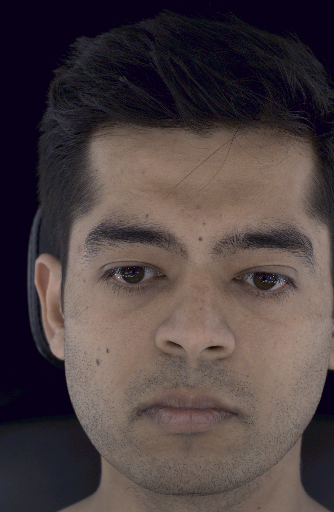
\includegraphics[width=\imagewidth,trim={1.2cm 0 0 0},clip]{assets/\blendfieldsdirname/data/gt/002757580_28_0.png} \&
            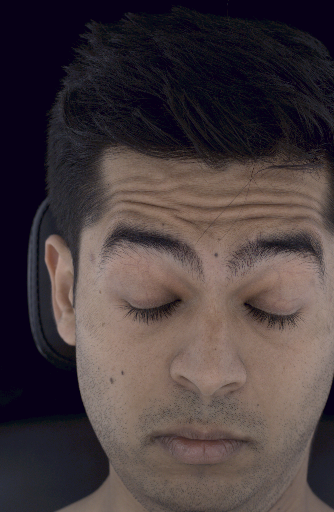
\includegraphics[width=\imagewidth,trim={1.2cm 0 0 0},clip]{assets/\blendfieldsdirname/data/gt/002757580_28_1.png} \&
            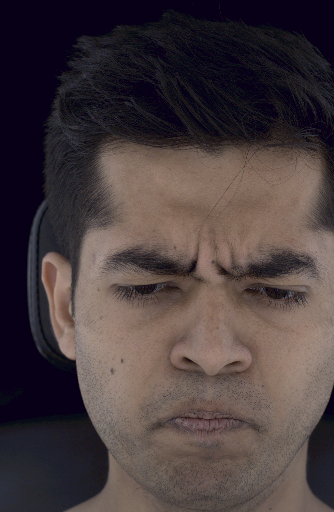
\includegraphics[width=\imagewidth,trim={1.2cm 0 0 0},clip]{assets/\blendfieldsdirname/data/gt/002757580_28_3.png} \&
            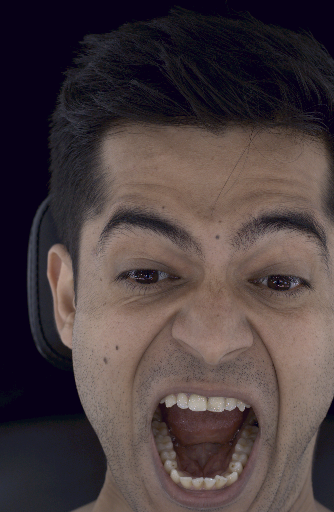
\includegraphics[width=\imagewidth,trim={1.2cm 0 0 0},clip]{assets/\blendfieldsdirname/data/gt/002757580_28_4.png} \\ % \&
            % \includegraphics[width=\imagewidth]{assets/data/gt/002757580_28_7.png}
            % \\
          };
          \node[below right=\offset and \offset of datarep-1-1.north west, overlay]{
            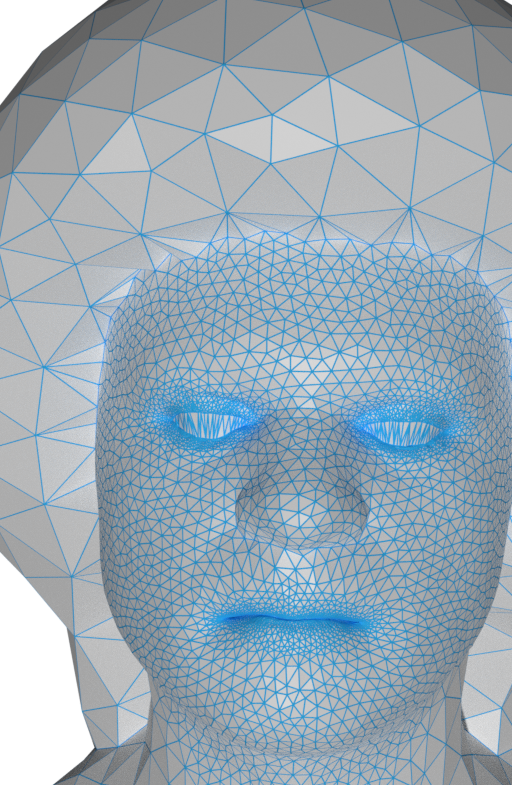
\includegraphics[width=\smallimagewidth]{assets/\blendfieldsdirname/data/wireframes/mesh_frame_0.png}
          };
          \node[below right=\offset and \offset of datarep-1-2.north west, overlay]{
            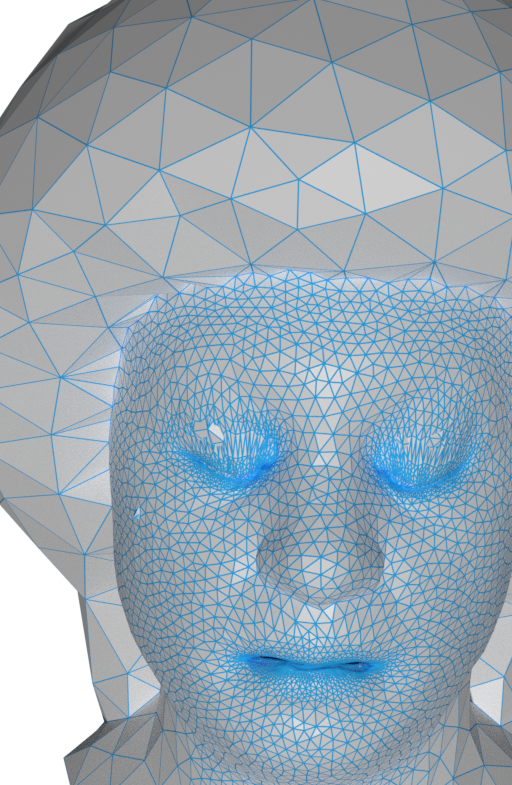
\includegraphics[width=\smallimagewidth]{assets/\blendfieldsdirname/data/wireframes/mesh_frame_1.png}
          };
          \node[below right=\offset and \offset of datarep-1-3.north west, overlay]{
            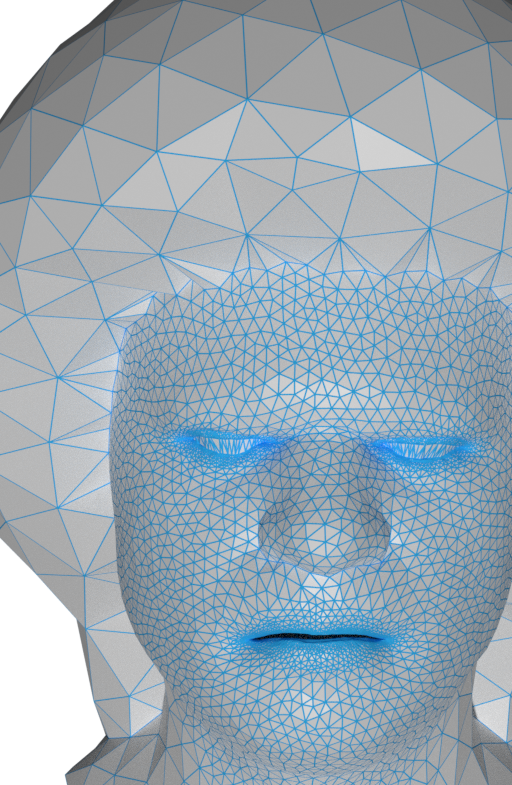
\includegraphics[width=\smallimagewidth]{assets/\blendfieldsdirname/data/wireframes/mesh_frame_3.png}
          };
          \node[below right=\offset and \offset of datarep-1-4.north west, overlay]{
            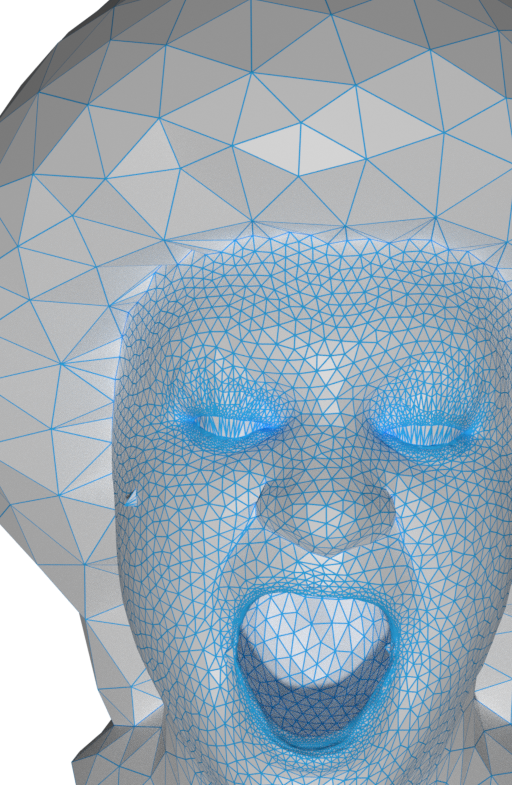
\includegraphics[width=\smallimagewidth]{assets/\blendfieldsdirname/data/wireframes/mesh_frame_4.png}
          };
          % \node[below right=\offset and \offset of datarep-1-5.north west,
          % overlay]{
          % \includegraphics[width=\smallimagewidth]{assets/data/wireframes/mesh_frame_7.png}
          % };
        \end{tikzpicture}
      }
    \end{subfigure}
  }
  \caption{\textbf{Data} -- We represent the data as a multi-view, multi-expression images.
    For each of these images, we obtain parameters of a parametric model, such
    as FLAME \cite{li2017flame} to get: an expression vector $\expression$ and
    a tetrahedral mesh described by vertices $\meshVertices(\expression)$.
    We highlight that our approach works for any object if a rough mesh and
    its descriptor are already provided.
  }
  \label{fig:blendfields-data-representation}
\end{figure}
    \noindent\textbf{Training the model}
    We train our model by assuming that we have access to a small set of $\nExpr$ images~$\{\image_\iExpr\}$ (example in \cref{fig:blendfields-data-representation}), each corresponding to an ``extreme'' expression $\{\expression_\iExpr\}$, and minimize the loss:
    \begin{align}
      \label{eq:blendfields-loss}
      \loss{rgb} & =
      \expect_{\iExpr} \:
      \expect_{\ray} \:
      \| \pixelcolor_\nExpr(\ray; \expression_\iExpr) - \pixelcolor_\iExpr(\ray) \|_2^2
      \\
                 & \text{where} \quad \forall \pos,\:\: \blendfield(\pos) = \indicator_\iExpr,
    \end{align}
    where $\indicator_\iExpr$ is the indicator vector, which has value one at the $k$-th position and zeroes elsewhere, and $\pixelcolor_\nExpr$ represents the output of integrating the radiances in~\cref{eq:blendfields-multiheadradiance} along a ray.
    % \AT{and what about the map function? I assume the expressions are stored
    % in canonical space too? Adjust the math to match}.\KK{Essentially yes.
    % Each of \auxcolor come from a mapping where points are first
    % canonicalized and then the branch \texttt{auxiliary} predicts set of
    % \auxcolor}/images

    % --- how we use it
    \noindent\textbf{Driving the model}
    To control our model given a novel expression $\expression$, we need to
    map the input expression code to the corresponding
    blendfield~$\blendfield(\pos)$.
    We parameterize the blend field as a vector field discretized on the
    vertices $\meshVertices(\expression)$ of our tetrahedral mesh, where the
    vertices deform according to the given expression.
    The field is discretized on vertices, but it can be queried within
    tetrahedra using linear FEM bases~\cite{monk2003finite}.
    % --- geometry 
    Our core intuition is that when the~(local) geometry of the mesh matches
    the local geometry in one of the input expressions, the corresponding
    expression blend weight should be locally activated.
    More formally, let $\vertex{\in} \meshVertices$ be a vertex in the tetrahedra and $\tetgeometry(\vertex)$ a local measure of volume on the vertex described in~\cref{sec:blendfields-similarity}, then
    \begin{align}
      \tetgeometry(\vertex(\expression)) {\approx} \tetgeometry(\vertex(\expression_\iExpr))
      \Longrightarrow
      \blendfield(\vertex(\expression)) \approx \indicator_\iExpr.
      \label{eq:blendfields-coreidea}
    \end{align}
    % \ve{I changed the order of the previous sentences to start with the
    % intuition in the first sentence and introduce notation in the second one.
    % } 
    To achieve this we first define a \textit{local} similarity measure:
    \begin{equation}
      \label{eq:blendfields-local-similarity}
      [ \Delta\tetgeometry_k(\vertex(\expression))] = [ \| \tetgeometry(\vertex(\expression)) {-} \tetgeometry(\vertex(\expression_\iExpr))\|_2^2 ] \in \real^{\nExpr}
    \end{equation}
    and then gate it with softmax (with temperature $\temp{=}10^6$) to obtain vertex blend weights:
    \begin{align}
      \label{eq:blendfields-blendfield}
      \blendfield(\vertex(\expression)) = \text{softmax}_\temp \{ \Delta\tetgeometry_k(\vertex(\expression)) \} \in [0,1]^{\nExpr}
    \end{align}
    which realizes~\cref{eq:blendfields-coreidea}, as well as preserves the typically desirable characteristics of blend weights:
    \begin{itemize}
      \item \textit{partition of unity}: $\forall\pos \:\: \blendfield(\pos) \in [0,1]^\nExpr$ and $\| \blendfield(\pos) \|_1{=}1$
      \item \textit{activations sparsity}: minimizers of $\|\blendfield(\pos)\|_0$
    \end{itemize}
    where the former ensures any reconstructed result is a~\textit{convex} combination of input data, and the latter prevents destructive interference~\cite{ichim2015dynamic}.

  \subsection{Local geometry descriptor}
    \label{sec:blendfields-similarity}
    Let us consider a tetrahedron as the matrix formed by its vertices~$\tet
    {=} \{\vertex_i\} \in \real^{3 \times 4}$, and its edge matrix as
    $\edgematrix = [\vertex_3-\vertex_0, \vertex_2-\vertex_0,
    \vertex_1-\vertex_0]$.
    Let us denote $\template\edgematrix$ as the edge matrix in rest pose and
    $\edgematrix$ as one of the deformed tetrahedra (\ie, due to expression).
    From classical FEM literature, we can then compute the change in volume of the tetrahedra from the determinant of its deformation gradient~\cite{irving2004invertible}:
    \begin{equation}
      \label{eq:blendfields-volume}
      \Delta \volume(\tet) = \text{det}(\edgematrix \cdot \template\edgematrix^{-1})
    \end{equation}
    We then build a local volumetric descriptor for a specific (deformed) vertex $\vertex(\expression)$ by concatenating the changes in volumes of neighboring (deformed) tetrahedra:
    \begin{align}
      \label{eq:blendfields-local-descriptor}
      \tetgeometry(\vertex(\expression)) =
      \bigoplus_{\tet \in \neighbourhood(\vertex)}
      \Delta \volume(\tet(\expression)),
    \end{align}
    where $\bigoplus$ denotes concatenation and $\neighbourhood(\vertex)$ topological neighborhood of a vertex $\vertex$.
    % \ve{I added the sentence after the equation to explain notation, Kacper
    % can you confirm that we use topological neighbours. This is what we did
    % last time I checked.}

    \begin{figure}[t]
  \centering
  \begin{overpic}[width=0.5\linewidth, trim=0 0 -1.3em -1em, clip]{assets/\blendfieldsdirname/laplacian.png}
    \put(11,98) {GT image}
    \put(37,98) {No smoothing}
    \put(65,98) {With smoothing}
    \put(95,79) {\rotatebox{-90}{RGB}}
    \put(95,46) {\rotatebox{-90}{$\blendfield(\pos)$ space (\cref{eq:blendfields-blendfield})}}
  \end{overpic}
  \caption{\textbf{Laplacian smoothing} -- To combat artifacts stemming from calculating weights $\blendingweight$ across multiple expressions, which may assign different expressions to neighboring tetrahedra, we apply Laplacian smoothing~\cite{desbrun1999implicit}.
    As seen in the bottom row, smoothing gives a more consistent expression
    assignment.
  }
  \label{fig:blendfields-laplacian-smoothing}
\end{figure}
    % 
\renewcommand{\imagewidth}{2.3cm}
\renewcommand{\imageheight}{4.0263671874999996cm}
\renewcommand{\smallimagewidth}{0.8cm}
\newcommand{\expressionsep}{0em}

\newcommand{\imageoneindex}[2]{
  \includegraphics[height=\imageheight, trim={0 0 0 0}, clip]{assets/\blendfieldsdirname/qualitative/main_v2/#1_6795937_extrapolation_#2.png}
}
\newcommand{\imagetwoindex}[2]{
  \includegraphics[height=\imageheight, trim={0 0 0 0}, clip]{assets/\blendfieldsdirname/qualitative/main_v2/#1_7889059_extrapolation_#2.png}
}
\renewcommand{\versionone}{
  \begin{tikzpicture}[
      >=stealth',
      overlay/.style={
          anchor=south west,
          draw=black,
          rectangle,
          line width=0.8pt,
          outer sep=0,
          inner sep=0,
        },
    ]
    \matrix[
      matrix of nodes,
      column sep=0pt,
      row sep=0pt,
      ampersand replacement=\&,
      inner sep=0,
      outer sep=0,
    ] (voltemorphstaticone) {
      \imageoneindex{voltemorph_static}{0000} \&
      \imageoneindex{voltemorph_static}{0002} \\
    };

    \matrix[
      matrix of nodes,
      column sep=0pt,
      row sep=0pt,
      ampersand replacement=\&,
      inner sep=0,
      outer sep=0,
      right=\expressionsep of voltemorphstaticone
    ] (voltemorphstatictwo) {
      \imagetwoindex{voltemorph_static}{0000} \&
      \imagetwoindex{voltemorph_static}{0002} \\
    };

    \matrix[
      matrix of nodes,
      column sep=0pt,
      row sep=0pt,
      ampersand replacement=\&,
      inner sep=0,
      outer sep=0,
      below=0pt of voltemorphstaticone
    ] (voltemorphone) {
      \imageoneindex{voltemorph}{0000} \&
      \imageoneindex{voltemorph}{0002} \\
    };

    \matrix[
      matrix of nodes,
      column sep=0pt,
      row sep=0pt,
      ampersand replacement=\&,
      inner sep=0,
      outer sep=0,
      right=\expressionsep of voltemorphone
    ] (voltemorphtwo) {
      \imagetwoindex{voltemorph}{0000} \&
      \imagetwoindex{voltemorph}{0002} \\
    };

    \matrix[
      matrix of nodes,
      column sep=0pt,
      row sep=0pt,
      ampersand replacement=\&,
      inner sep=0,
      outer sep=0,
      below=0pt of voltemorphone
    ] (oursone) {
      \imageoneindex{blendvolumes_aux}{0000} \&
      \imageoneindex{blendvolumes_aux}{0002} \\
    };

    \matrix[
      matrix of nodes,
      column sep=0pt,
      row sep=0pt,
      ampersand replacement=\&,
      inner sep=0,
      outer sep=0,
      right=\expressionsep of oursone
    ] (ourstwo) {
      \imagetwoindex{blendvolumes_aux}{0000} \&
      \imagetwoindex{blendvolumes_aux}{0002} \\
    };
    \node[above=0.0em of voltemorphstaticone-1-1.north, align=center, anchor=south]{Neutral};
    \node[above=0.0em of voltemorphstaticone-1-2.north, align=center, anchor=south]{Frowned and Smiled};

    \node[above=0.0em of voltemorphstatictwo-1-1.north, align=center, anchor=south]{Neutral};
    \node[above=0.0em of voltemorphstatictwo-1-2.north, align=center, anchor=south]{Eyes Squint, Lips Moved Left};

    % \node[above=0.0em of voltemorphone-1-1.north, align=center,
    % anchor=south]{Neutral}; \node[above=0.0em of voltemorphone-1-2.north,
    % align=center, anchor=south]{Eyes Squint, Lips Moved Left};

    % \node[above=0.0em of hypernerfstatic-1-1.north, align=center,
    % anchor=south]{HyperNeRF-AP}; \node[above=0.0em of
    % hypernerfdynamic-1-1.north, align=center, anchor=south]{HyperNeRF-DS};
    % \node[above=0.0em of voltemorphstatic-1-1.north, align=center,
    % anchor=south]{VolTeMorph$^\dagger$}; \node[above=0.0em of
    % voltemorph-1-1.north, align=center, anchor=south]{VolTeMorph};
    % \node[above=0.2em of ours-1-1.north, align=center,
    % anchor=south]{\textbf{Ours}};

    % \node[left=0em of voltemorphstaticone-1-1.west, align=center,
    % anchor=east]{\rotatebox{90}{Neutral}}; \node[left=0em of nerf-3-1.west,
    % align=center, anchor=east]{\rotatebox{90}{Neutral}};

    % \node[left=0em of nerf-2-1.west, align=center,
    % anchor=east]{\rotatebox{90}{Frowned and Smile}}; \node[left=0em of
    % nerf-4-1.west, align=center, anchor=east]{\rotatebox{90}{Eyes Squint,
    % Lips Moved Left}};

    \node[left=0em of voltemorphstaticone-1-1.west, align=center, anchor=east]{\rotatebox{90}{VolTeMorph$_1$}};
    \node[left=0em of voltemorphone-1-1.west, align=center, anchor=east]{\rotatebox{90}{VolTeMorph$_\text{avg}$}};
    \node[left=0em of oursone-1-1.west, align=center, anchor=east]{\rotatebox{90}{\textbf{Ours}}};

    % \node[left=0em of nerf-2-1.west, align=center,
    % anchor=east]{\rotatebox{90}{Frowned and Smile}}; \node[left=0em of
    % nerf-4-1.west, align=center, anchor=east]{\rotatebox{90}{Eyes Squint,
    % Lips Moved Left}};
  \end{tikzpicture}
}

\begin{figure*}[htb]
  \centering
  \resizebox{\linewidth}{!}{
    \versionone
  }
  \caption{\textbf{Novel expression synthesis} -- {
      We compare qualitatively \blendfields with selected baselines (vertical)
      across two selected subjects (horizontal).
      To our surprise, VolTeMorph$_\text{avg}$ trained on multiple frames
      renders some details too but with much lower fidelity.
      We argue that VolTeMorph considers rendering wrinkles as artifacts that
      depend on the view direction
      (see~\cref{eq:blendfields-rendering-equation}).
      VolTeMorph$_1$ is limited to producing wrinkles it was trained for.
      In contrast to those baselines, \textbf{\blendfields} captures the
      details and generalizes outside of the distribution.
      Please refer to the \supplementary{} for animated sequences and results
      for other methods.
    }}
  \label{fig:blendfields-qualitative-comparison}
\end{figure*}
    
\renewcommand{\imagewidth}{2.3cm}
\renewcommand{\imageheight}{4.0263671874999996cm}
\renewcommand{\smallimagewidth}{0.8cm}
\newcommand{\expressionsep}{0em}

\newcommand{\imageoneindex}[2]{
  \includegraphics[height=\imageheight, trim={0 0 0 0}, clip]{assets/\blendfieldsdirname/qualitative/main_v2/#1_6795937_extrapolation_#2.png}
}
\newcommand{\imagetwoindex}[2]{
  \includegraphics[height=\imageheight, trim={0 0 0 0}, clip]{assets/\blendfieldsdirname/qualitative/main_v2/#1_7889059_extrapolation_#2.png}
}
\newcommand{\versionone}{
  \tikzsetnextfilename{blendfields_comparison_v2}
  \begin{tikzpicture}[
      >=stealth',
      overlay/.style={
          anchor=south west,
          draw=black,
          rectangle,
          line width=0.8pt,
          outer sep=0,
          inner sep=0,
        },
    ]
    \matrix[
      matrix of nodes,
      column sep=0pt,
      row sep=0pt,
      ampersand replacement=\&,
      inner sep=0,
      outer sep=0
    ] (gt) {
      \imageoneindex{gt}{0505} \&
      \imageoneindex{gt}{0000} \&
      \imagetwoindex{gt}{0000} \&
      \imagetwoindex{gt}{0852} \\
    };
    \matrix[
      matrix of nodes,
      column sep=0pt,
      row sep=0pt,
      ampersand replacement=\&,
      inner sep=0,
      outer sep=0,
      below=0pt of gt,
    ] (voltemorphstatic) {
      \imageoneindex{voltemorph_static}{0505} \&
      \imageoneindex{voltemorph_static}{0000} \&
      \imagetwoindex{voltemorph_static}{0000} \&
      \imagetwoindex{voltemorph_static}{0852} \\
    };

    \matrix[
      matrix of nodes,
      column sep=0pt,
      row sep=0pt,
      ampersand replacement=\&,
      inner sep=0,
      outer sep=0,
      below=0pt of voltemorphstatic
    ] (voltemorph) {
      \imageoneindex{voltemorph}{0505} \&
      \imageoneindex{voltemorph}{0000} \&
      \imagetwoindex{voltemorph}{0000} \&
      \imagetwoindex{voltemorph}{0852} \\
    };

    \matrix[
      matrix of nodes,
      column sep=0pt,
      row sep=0pt,
      ampersand replacement=\&,
      inner sep=0,
      outer sep=0,
      below=0pt of voltemorph
    ] (ours) {
      \imageoneindex{bv_aux}{0505} \&
      \imageoneindex{bv_aux}{0000} \&
      \imagetwoindex{bv_aux}{0000} \&
      \imagetwoindex{bv_aux}{0852} \\
    };

    \node[left=0em of gt-1-1.west, align=center, anchor=east]{\rotatebox{90}{Ground Truth}};
    \node[left=0em of voltemorphstatic-1-1.west, align=center, anchor=east]{\rotatebox{90}{VolTeMorph$_1$}};
    \node[left=0em of voltemorph-1-1.west, align=center, anchor=east]{\rotatebox{90}{VolTeMorph$_\text{avg}$}};
    \node[left=0em of ours-1-1.west, align=center, anchor=east]{\rotatebox{90}{\textbf{Ours}}};

    \node[above=0em of gt-1-1.north, align=center, anchor=south]{Neutral};
    \node[above=0em of gt-1-2.north, align=center, anchor=south]{Posed};
    \node[above=0em of gt-1-3.north, align=center, anchor=south]{Neutral};
    \node[above=0em of gt-1-4.north, align=center, anchor=south]{Posed};
  \end{tikzpicture}
}

\begin{figure*}[htb]
  \centering
  \resizebox{\linewidth}{!}{\versionone}
  \caption{\textbf{Novel expression synthesis} --
    We compare qualitatively \blendfields with selected baselines (vertical) across two selected subjects (horizontal).
    Firstly, we show a neutral pose of the subject and then any of the
    available expressions.
    To our surprise, VolTeMorph$_\text{avg}$ trained on multiple frames
    renders some details but with much lower fidelity.
    We argue that VolTeMorph$_\text{arg}$ considers rendering wrinkles as
    artifacts that depend on the view direction
    (see~\cref{eq:blendfields-rendering-equation}).
    VolTeMorph$_1$ is limited to producing the wrinkles it was trained for.
    In contrast to those baselines, \textbf{\blendfields} captures the details
    and generalizes outside of the distribution.
    Please refer to the \supplementary{} for animated sequences and results
    for other methods.
  }
  \label{fig:blendfields-qualitative-comparison}
\end{figure*}
    % \renewcommand{\imagewidth}{2.3cm}
\renewcommand{\imageheight}{3.5263671874999996cm}
\renewcommand{\smallimagewidth}{0.8cm}

\newcommand{\indexone}{0521}
\newcommand{\indextwo}{0377}
\newcommand{\indexthree}{0453}
\newcommand{\indexfour}{0854}

\newcommand{\imageone}[1]{
  \includegraphics[height=\imageheight, trim={0.7cm 1.2cm 0 0}, clip]{assets/\blendfieldsdirname/qualitative/main/#1_2183941_rom_\indexone}
}
\newcommand{\imagetwo}[1]{
  \includegraphics[height=\imageheight, trim={0.7cm 1.2cm 0 0}, clip]{assets/\blendfieldsdirname/qualitative/main/#1_5372021_rom_\indextwo}
}
\newcommand{\imagethree}[1]{
  \includegraphics[height=\imageheight, trim={0.7cm 1.2cm 0 0}, clip]{assets/\blendfieldsdirname/qualitative/main/#1_6795937_rom_\indexthree}
}
\newcommand{\imagefour}[1]{
  \includegraphics[height=\imageheight, trim={0.7cm 1.2cm 0 0}, clip]{assets/\blendfieldsdirname/qualitative/main/#1_7889059_rom_\indexfour}
}

\newcommand{\imageoneindex}[2]{
  \includegraphics[height=\imageheight, trim={0.7cm 1.2cm 0 0}, clip]{assets/\blendfieldsdirname/qualitative/main/#1_2183941_rom_#2}
}
\newcommand{\imagetwoindex}[2]{
  \includegraphics[height=\imageheight, trim={0.7cm 1.2cm 0 0}, clip]{assets/\blendfieldsdirname/qualitative/main/#1_5372021_rom_#2}
}
\newcommand{\imagethreeindex}[2]{
  \includegraphics[height=\imageheight, trim={0.7cm 1.2cm 0 0}, clip]{assets/\blendfieldsdirname/qualitative/main/#1_6795937_rom_#2}
}
\newcommand{\imagefourindex}[2]{
  \includegraphics[height=\imageheight, trim={0.7cm 1.2cm 0 0}, clip]{assets/\blendfieldsdirname/qualitative/main/#1_7889059_rom_#2}
}

\newcommand{\versionthree}{
  \tikzsetnextfilename{blendfields_comparison}
  \tikzset{external/export next=false}
  \begin{tikzpicture}[
      >=stealth',
      overlay/.style={
          anchor=south west,
          draw=black,
          rectangle,
          line width=0.8pt,
          outer sep=0,
          inner sep=0,
        },
    ]
    \matrix[
      matrix of nodes,
      column sep=0pt,
      row sep=0pt,
      ampersand replacement=\&,
      inner sep=0,
      outer sep=0,
    ] (gt) {
      \imageoneindex{gt}{0190} \&
      \imageoneindex{gt}{0521} \&
      \imagetwoindex{gt}{0377} \&
      \imagetwoindex{gt}{0638} \&
      \imagethreeindex{gt}{0453} \&
      \imagethreeindex{gt}{0735} \&
      \imagefourindex{gt}{0854} \&
      \imagefourindex{gt}{1018} \\
    };

    \matrix[
      matrix of nodes,
      column sep=0pt,
      row sep=0pt,
      ampersand replacement=\&,
      inner sep=0,
      outer sep=0,
      below=0pt of gt
    ] (voltemorphstatic) {
      \imageoneindex{voltemorph_static}{0190} \&
      \imageoneindex{voltemorph_static}{0521} \&
      \imagetwoindex{voltemorph_static}{0377} \&
      \imagetwoindex{voltemorph_static}{0638} \&
      \imagethreeindex{voltemorph_static}{0453} \&
      \imagethreeindex{voltemorph_static}{0735} \&
      \imagefourindex{voltemorph_static}{0854} \&
      \imagefourindex{voltemorph_static}{1018} \\
    };

    \matrix[
      matrix of nodes,
      column sep=0pt,
      row sep=0pt,
      ampersand replacement=\&,
      inner sep=0,
      outer sep=0,
      below=0pt of voltemorphstatic
    ] (voltemorph) {
      \imageoneindex{voltemorph}{0190} \&
      \imageoneindex{voltemorph}{0521} \&
      \imagetwoindex{voltemorph}{0377} \&
      \imagetwoindex{voltemorph}{0638} \&
      \imagethreeindex{voltemorph}{0453} \&
      \imagethreeindex{voltemorph}{0735} \&
      \imagefourindex{voltemorph}{0854} \&
      \imagefourindex{voltemorph}{1018} \\
    };

    \matrix[
      matrix of nodes,
      column sep=0pt,
      row sep=0pt,
      ampersand replacement=\&,
      inner sep=0,
      outer sep=0,
      below=0pt of voltemorph
    ] (blendvolumes) {
      \imageoneindex{blendvolumes_aux}{0190} \&
      \imageoneindex{blendvolumes_aux}{0521} \&
      \imagetwoindex{blendvolumes_aux}{0377} \&
      \imagetwoindex{blendvolumes_aux}{0638} \&
      \imagethreeindex{blendvolumes_aux}{0453} \&
      \imagethreeindex{blendvolumes_aux}{0735} \&
      \imagefourindex{blendvolumes_aux}{0854} \&
      \imagefourindex{blendvolumes_aux}{1018} \\
    };

    \node[left=0.0em of gt.west, align=center, anchor=east]{\rotatebox{90}{GT}};
    \node[left=0.0em of voltemorphstatic.west, align=center, anchor=east]{\rotatebox{90}{VolTeMorph$^\dagger$~\cite{garbin2024voltemorph}}};
    \node[left=0.0em of voltemorph.west, align=center, anchor=east]{\rotatebox{90}{VolTeMorph~\cite{garbin2024voltemorph}}};
    \node[left=0.1em of blendvolumes.west, align=center, anchor=east]{\rotatebox{90}{\textbf{Ours}}};
  \end{tikzpicture}
}
\begin{figure}[t]
  \centering
  \resizebox{\linewidth}{!}{
    \versionthree
  }
  % \includegraphics[height=0.75\textheight, width=\linewidth]{example-image-a}
  \caption{\textbf{Qualitative comparison} --
    We compare qualitatively \blendfields with selected baselines
    (horizontal) across used datasets (vertical).
    As clearly seen, our approach renders the most realistic frames given any
    of the expressions.
    VolTeMorph, while being capable of rendering already realistic, controlled
    images, it cannot capture expression-dependent details.
    In contrast, \blendfields captures these details and generalizes outside
    of the distribution.
  }
  \label{fig:blendfields-qualitative-comparison}
\end{figure}
  \subsection{Blend-field smoothness}
    \label{sec:blendfields-smoothness}
    \newcommand{\blendfieldVertices}{\mathbf{A}}
    High-frequency spatial changes in blendfields can cause visual artifacts,
    see~\cref{fig:blendfields-laplacian-smoothing}.
    We overcome this issue by applying a small amount of smoothing to the
    blendfield.
    Let us denote with $\blendfieldVertices{=}\{\blendfield(\vertex_v)\}$ the
    matrix of blend fields defined on all mesh vertices, and with $\mathbf{L}$
    the Laplace-Beltrami operator for the tetrahedral mesh induced by linear
    bases~\cite{irving2004invertible}.
    % \AT{wrong reference, this is linear bases on tri-meshes, not tet-meshes!}
    We exploit the fact that at test-time, the field is discretized on the mesh vertices, execute a diffusion process on the tetrahedral manifold, and, to avoid instability problems, implement it via backward Euler~\cite{desbrun1999implicit}:
    \begin{equation}
      \blendfieldVertices^\text{diff} = (\mathbf{I} - \hyperparam_\text{diff} \laplacian)^{-1} \blendfieldVertices^n.
    \end{equation}

  \subsection{Implementation details}
    \label{sec:blendfields-implementation}
    We build on VolTeMorph~\cite{garbin2024voltemorph} and use its volumetric
    3DMM face model.
    However, the same methodology can be used with other tetrahedral cages
    built on top of 3DMM face models.
    The face model is created by extending the blendshapes of the parametric
    3DMM face model~\cite{wood2021fake} to a tetrahedral cage that defines the
    support in the neural radiance field.
    It has four bones controlling global rotation, the neck and the eyes with
    linear blend skinning, 224 expression blendshapes, and 256 identity
    blendshapes.
    Our face radiance fields are thus controlled and posed with the identity,
    expression, and pose parameters of the 3DMM face
    model~\cite{wood2021fake}, can be estimated by a real-time face tracking
    system like~\cite{wood20223d}, and generalize convincingly to expressions
    representable by the face model.

    \noindent\textbf{Training.}
    During training, we sample rays from a single frame to avoid out-of-memory
    issues when evaluating the tetrahedral mesh for multiple frames.
    Each batch contains~1024 rays.
    We sample $\coarsesamples{=}128$ points along a single ray during the
    coarse sampling and $\importancesamples{=}64$ for the importance sampling.
    We train the network to minimize the loss in~\cref{eq:blendfields-loss}
    and sparsity losses with standard weights used in
    VolTeMorph~\cite{garbin2024voltemorph,hedman2021baking}.
    We train the methods for~$5{\times}10^5$ steps using
    Adam~\cite{kingma2014adam} optimizer with learning rate~$5{\times}10^{-4}$
    decaying exponentially by factor of~$0.1$ every~$5{\times}10^5$ steps.

    \noindent\textbf{Inference.}
    During inference, we leverage the underlying mesh to sample points around
    tetrahedra hit by a single ray.
    Therefore, we perform a single-stage sampling with
    $\numberofsamples{=}\coarsesamples{+}\importancesamples$ samples along the
    ray.
    When extracting the features~(\cref{eq:blendfields-local-descriptor}), we
    consider $|\neighbourhood(\vertex)|{=}20$ neighbors.
    For the Laplacian smoothing, we set $\weightdiffusion{=}0.1$ and perform a
    single iteration step.
    Geometric-related operations impose negligible computational overhead.
    % These steps require two evaluations of NeRF networks
    % (see~\cref{fig:pipeline}), 
